\documentclass{standalone}
\usepackage{tikz}

\begin{document}

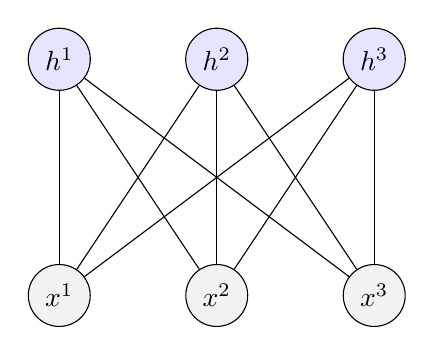
\begin{tikzpicture}
  \tikzset{
    hnode/.style={
      draw, circle, fill=blue!10
    },
    xnode/.style={
      hnode, fill=gray!10
    }
  }

  \foreach \i in {1, ..., 3} {
    \node [hnode] (h\i) at (\i*2, 3) {$h^\i$};
    \node [xnode] (x\i) at (\i*2, 0) {$x^\i$};
  }

  % this has to be a separate loop b/c the node has to exist before the path is drawn
  \foreach \i in {1, ..., 3} {
    \foreach \j in {1, ..., 3} {
      \path (h\i) edge [draw] (x\j);
    }
  }
\end{tikzpicture}

\end{document}
